Our method has to be illustrated with a simplest example, namely three-jet production at lepton-collider $ e^+ e^- \rightarrow q + \bar{q} + g $. As shown in section \ref{Parton showers}, at first perturbative order, two Feynman diagrams contribute to the matrix element corresponding to the emission of a gluon from either the final-state quark or the anti-quark. The partonic differential cross section with respect to the quark and anti-quark momentum fractions was given by \ref{fully}:
\begin{equation}
\frac{d^2 \sigma}{dx_1 dx_2}= \hat{\sigma_0}
\frac{\alpha_s}{2\pi} C_F \frac{{x_1}^2+{x_2}^2}{(1-x_1)(1-x_2)}
\label{confi}
\end{equation}

In the parton shower approach, two contributions occur as well. For the final result, those two contributions have to be summed. 

\begin{figure}[h!]
\centering
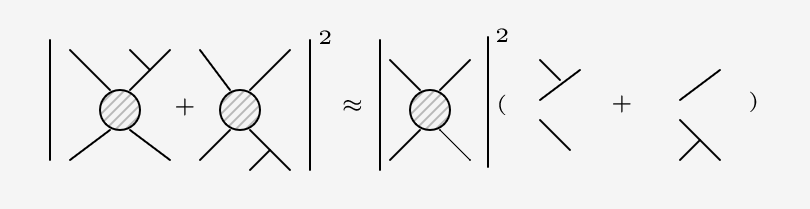
\includegraphics[width=0.85\textwidth]{images/Intro/factorization.png}
\caption{Dipole/Antenna factorisation}
\end{figure}


The dipole factorisation formula is defined by:

 \begin{equation}
 |\mathcal{M}_m+1|^2 = \displaystyle\sum\limits_{i,j} \displaystyle\sum\limits_{k\neq i,j} \mathcal{D}_{ij,k} +\displaystyle\sum\limits_{i,j} \displaystyle\sum\limits_{a} {\mathcal{D}^a}_{ij}+\displaystyle\sum\limits_{a,i} \displaystyle\sum\limits_{k\neq i} {\mathcal{D}^{ai}}_{k}+\displaystyle\sum\limits_{a,i} \displaystyle\sum\limits_{b\neq a} \mathcal{D}^{aj,b}+...
 \end{equation}
 
The calculation of the subtracted cross section involves just the evaluation of two dipole contributions from the final state emitter and final-state spectator (FF), which are $ D_{13,2} $ and $ D_{23,1} $. 

\begin{equation}
\begin{split}
\mathcal{D}_{13,2} (q_i,q_j,q)&= \frac{-1}{2q_i \cdot q} \:\:_2<1,\tilde{13},\tilde{2} |\frac{T_2 \cdot T_{13}}{{T_{13}}^2} V_{13,2}| 1,\tilde{13},\tilde{2} >\:_2\\
\mathcal{D}_{13,2} (q_i,q_j,q)&=\frac{1}{2p_i \cdot p_j} V_{13,2} |\mathcal{M}_{2}|^2
\end{split}
\end{equation}



\begin{equation}
\begin{split}
\mathcal{D}_{13,2} (q_i,q_j,q) &= \frac{1}{2p_i \cdot p_j}[\frac{(d-2)(1-z)(1-y) }{y}+\frac{(d-2)yz^2}{(1-z)(1-y)}(\frac{-2z}{z-1}) \frac{1}{y}]|\mathcal{M}_{2}|^2
\end{split}
\end{equation}

In collinear limits one obtaines:

\begin{equation}
\begin{split}
\mathcal{D}_{13,2} (q_i,q_j,q) &= \frac{1}{2yp_i \cdot p_j}[\epsilon(1-z)+(\frac{z^2+1}{z-1})]|\mathcal{M}_{2}|^2
\end{split}
\end{equation}

For simplicity $ \epsilon \rightarrow 0 $:
\begin{equation}
\begin{split}
\mathcal{D}_{13,2} (q_i,q_j,q) &= \frac{1}{2p_i \cdot p_j}[\frac{1}{y}\frac{z^2+1}{z-1}]|\mathcal{M}_{2}|^2
\end{split}
\end{equation}

In order to compare our result with the result from $ e^+ e^- $ annihilation the shower variables are introduced and expressed in terms of the energy fraction $ x_i=\frac{2 q_i \cdot Q}{Q^2} $.
To find the relationship between the variables, we define a total momentum $Q^{\mu} = (Q, \overrightarrow{0})$ in the Center of Mass frame.
From equation \ref{tot} it can be obtained:

\begin{equation}
\begin{split}
&p_i = Q/2\:(1, \overrightarrow{0}_\bot, 1)\\
&p_i = Q/2\:(1, \overrightarrow{0}_\bot, 1)
\end{split}
\end{equation}

So the desired relations can be achieved:

\begin{equation}
\begin{split}
x_1 &= z + y(1-z)\\
x_2 &= 1-y\\
x_3 &= (1-z)+yz
\label{ret}
\end{split}
\end{equation}
The addition of $x_i$ is 2 as already mentioned in section \ref{ir}.
hence, the shower variables are:

\begin{equation}
\begin{split}
&\tilde{z_1}=\frac{x_1+x_2-1}{x_2}\\
&y_{13,2} =1-x_2
\label{ex}
\end{split}
\end{equation}



For the gluon emission from the quark, after using the expressions \ref{ex} we get, following the logic from~\cite{Schumann:2007mg}:

\begin{equation}
\begin{split}
\frac{d^2 \sigma}{dx_1 dx_2}_{PS_q}&= \hat{\sigma_0}
\frac{\alpha_s}{2\pi} C_F [\frac{1}{y_{13,2}} (\frac{2}{1-\tilde{z_1}}-(1+\tilde{z_1})]\\
\Rightarrow \frac{d^2 \sigma}{dx_1 dx_2}_{PS_q}&= \hat{\sigma_0}
\frac{\alpha_s}{2\pi} C_F [\frac{1}{1-x_2} (\frac{2}{2-x_1-x_2}-(1+x_1))+\frac{1-x_1}{x_2}]
\end{split}
\end{equation}




For exactly the same calculation for a gluon emission of an anti-quark, there is no need to find $ D_{23,1} $. It is enough to swap $ x_1 $ with $ x_2 $:

\begin{equation}
\frac{d^2 \sigma}{dx_1 dx_2}_{PS_{\bar{q}}}= \hat{\sigma_0}
\frac{\alpha_s}{2\pi} C_F [\frac{1}{1-x_1} (\frac{2}{2-x_2-x_1}-(1+x_2))+\frac{1-x_2}{x_1}]
\end{equation}



Thus, the total parton shower cross section will be:

\begin{equation}
\frac{d^2 \sigma}{dx_1 dx_2}|_{PS}=\frac{d^2 \sigma}{dx_1 dx_2}|_{PS_q}+\frac{d^2 \sigma}{dx_1 dx_2}|_{PS_{\bar{q}}}= \hat{\sigma_0}
\frac{\alpha_s}{2\pi} C_F [\frac{{x_1}^2+{x_2}^2}{(1-x_1)(1-x_2)}+\frac{1-x_1}{x_2}+\frac{1-x_2}{x_1}]
\end{equation}

Obviously, the parton shower exactly reproduces the soft and collinear singular structure of the matrix element as $ x_{1,2} \rightarrow 1 $.


%%%%%%%%%%%%%%%%%%%%%  -------  4 images  -------  %%%%%%%%%%%%%%%%%%%%%
\begin{figure}[h!]
\begin{center}
\begin{minipage}{0.40\linewidth}
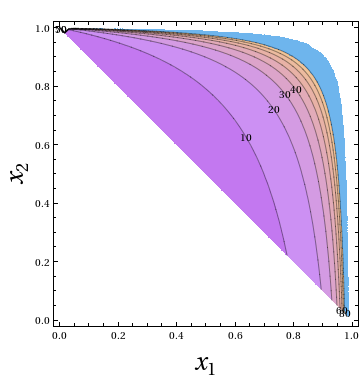
\includegraphics[width=\linewidth]{images/ms1.png}
\end{minipage}%
\hfill
\begin{minipage}{0.40\linewidth}
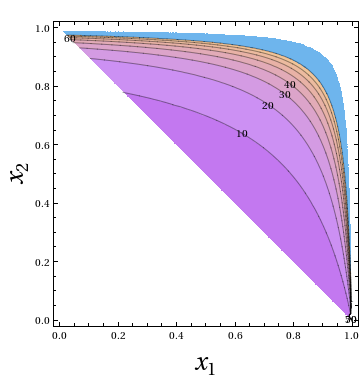
\includegraphics[width=\linewidth]{images/sw.png}
\end{minipage}
\end{center}
\begin{center}
\begin{minipage}{0.40\linewidth}
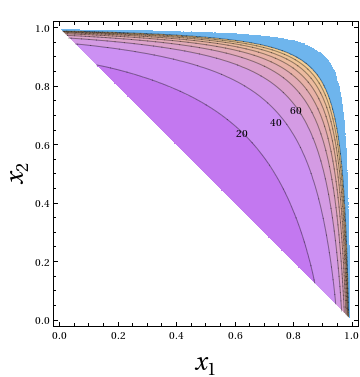
\includegraphics[width=\linewidth]{images/ms1undsw.png}
\end{minipage}
\hfill
\begin{minipage}{0.40\linewidth}
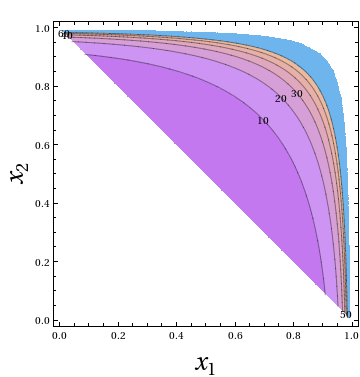
\includegraphics[width=\linewidth]{images/ann.png}
\end{minipage}
\captionof{figure}{Represented are cross sections  as contour plots in the phase space for the gluon emission from the quark (left top), gluon emission from the antiquark (right top), Additional case $ D_{13,2} $ and $ D_{23,1} $ (left bottom) and full calculation \ref{confi} (right bottom). As can be expected, the diagram from $ D_{13,2} $ is anti-symmetrical to the diagram $ D_{23,1} $, since the dipoles are obtained by swapping $ x_1 $ and $ x_2 $. It is remarkable that from the addition of the dipoles almost the same plot is achieved as in the full matrix element. The only difference is that the values on the contours of the dipole diagrams are larger and this can be explained by the extra contributions in the dipole matrix elements.}
\end{center}

\end{figure}


Our total results from the matrix of gluon radiation from an (anti)quark must actually give the same result as the equation \ref{confi}. Unfortunately, the full calculation can not be obtained because some  information about the behaviour of ${m^{\mu}}_{\bot}$ for the evaluation of the full matrix element are missing. But the result from the full matrix element and the outcome \ref{coll} in the collinear region can be compared. Therefore the full calculation is re-transformed with the relation \ref{ret} and finally the result will be exactly the same as in equation \ref{coll}.





